\documentclass[manuscript]{aastex62}
\usepackage{amsmath}
\usepackage{mathtools}
\usepackage{color}
\usepackage[normalem]{ulem}

\newcommand\latex{La\TeX}
\newcommand{\dd}{{\mathrm d}}
\newcommand{\rmsub}[1]{_\mathrm{#1}}
\newcommand{\bmu}{\boldsymbol{\mu}}
\newcommand{\beps}{\boldsymbol{\varepsilon}}
\newcommand{\blam}{\boldsymbol{\Lambda}}
\newcommand{\vx}[1]{{\bf {#1}}}
\newcommand{\vxhat}[1]{{\bf {\hat{#1}}}}

\graphicspath{{./}{figures/}}

\shorttitle{Multiplicative linear nuisance parameters}
\shortauthors{Tchernyshyov}

\begin{document}

\title{Analytic marginalization of absorption line continua and other multiplicative linear nuisance parameters}

\author[0000-0003-0789-9939]{Kirill Tchernyshyov}
\affiliation{Department of Physics and Astronomy, Johns Hopkins University, 3400 N. Charles Street, Baltimore, MD 21218, USA}
\correspondingauthor{Kirill Tchernyshyov}
\email{ktcherny@gmail.com}

%\author[0000-0003-4797-7030]{J. E. G. Peek}
%\affiliation{Department of Physics and Astronomy, Johns Hopkins University, 3400 N. Charles Street, Baltimore, MD 21218, USA}
%\affiliation{Space Telescope Science Institute, 3700 San Martin Drive, Baltimore, MD 21218, USA}

\begin{abstract}
absorption line fitting; speeding it up; well-motivated ways of selecting parameters; large spectroscopic surveys
\end{abstract}

\keywords{methods: statistical}

\section{Introduction}
\label{sec:introduction}
The formation and measurement of many astronomical observables involves processes that combine multiplicatively rather than additively.
Light from a distant source is attenuated by intervening interstellar matter (ISM) on its way to a detector; the output of the detector has to be converted to physically meaningful units by applying calibration factors.
Often, only some of the multiplicative processes represented in an observable are relevant to a study.
Attenuation by the ISM is a confounding variable for a study of a stellar populations based on a color magnitude diagram; the intrinsic spectral energy distribution of a star is a confounding variable in a study of the shape of the interstellar extinction curve.
When using Bayesian inference to learn about the relevant processes, it is necessary to marginalize over the parameters describing the confounding processes.
Because this marginalization can be time consuming if done using a numerical method such as Markov chain Monte Carlo (MCMC), it is advantageous to marginalize over nuisance parameters analytically whenever this is possible.
We have created a package, \texttt{name}\footnote{available \emph{here}}, for analytically marginalizing over nuisance parameters that enter an observable multiplicatively and linearly (multiplicative linear nuisance parameters or MLNPs).

The problem this package is designed for is the analysis of absorption features in spectra.
The process by which a spectrum containing absorption features is formed is the first example we gave in the paragraph above: a source emits light which is then attenuated by intervening matter.
The unattenuated light is customarily called \emph{the continuum}.
To determine parameters describing the intervening matter, it is necessary to also determine parameters describing the continuum.
While it is possible to pre-determine the continuum parameters using a portion of the spectrum that does not contain absorption features, we prefer to infer the absorption feature and continuum parameters simultaneously in order to explicitly include the uncertainty in continuum placement in estimates of the absorption feature parameters.
This is also the approach used in the recently released absorption line analysis packages \texttt{Starfish}, \texttt{sick}, and \texttt{BayesVP} \citep{2015ApJ...812..128C,2016ApJS..223....8C,Liang:2018kq}.
In these packages, absorption feature and continuum parameters are simultaneously marginalized over using MCMC.
The authors of both packages point out that marginalizing over large numbers of continuum parameters in this way can lead to long convergence and autocorrelation times.
To keep the number of continuum parameters low, the packages either do not support (\texttt{BayesVP}) or advise against (\texttt{sick}) including continuum parameters when simultaneously analyzing multiple spectral segments.

If the continuum is a linear function of the continuum parameters, the prior on the continuum parameters is (multivariate) normal or improper uniform, and the likelihood function of the observed spectrum given a model spectrum is multivariate normal, the necessary marginalization can be done analytically instead of numerically.
The key is that when the absorption feature parameters are held fixed, the continuum basis elements, the transmittance spectrum, and, if necessary, the line spread function (LSF) can be combined into a single design matrix.
The problem becomes equivalent to the simple linear nuisance parameter model discussed in an astronomical context in \citet{2017RNAAS...1a...7L}.
The likelihood marginalized over the continuum parameters is available in e.g. \citet{Rasmussen:2006vz} for both the normal prior and the improper uniform prior cases.

Analytic marginalization over multiplicative linear nuisance parameters has been used for other problems in astronomy.
In one common use case, the parameter that is marginalized over is the amplitude of a signal whose shape is a non-linear function of some parameters of interest.
One example of this use case is \citet{2017ApJ...837...20P}, where the parameters of interest are the period, eccentricity, phase, and argument of the radial velocity curve of a potential binary system and the nuisance parameters are the velocity amplitude of the curve and the barycenter velocity of the system.
Another example can be found in \citet{Leistedt:2017in}, where the parameter of interest is the redshift of a galaxy  and the nuisance parameter is the galaxy's luminosity.
This problem is not identical to the ones discussed in our paper and in \citet{2017ApJ...837...20P} because the luminosity multiplies both the data and the covariance matrix of the model residuals.
The resulting marginal likelihood can not be expressed in terms of commonly used functions.
The concept, however, is analogous and an accurate analytic approximation is available.

When developing this package, we were specifically considering properties of the absortion spectrum likelihood function and useful ways in which it can be factored.
The mathematical contribution of this work is an expression for the gradient of the logarithm of the marginal likelihood with respect to the problem's interesting non-linear parameters.
This gradient can be used for optimization or in gradient-aware sampling methods such as Hamiltonian Monte Carlo \citep{DUANE1987216}.
The other contribution is the package itself, which uses the structure of the likelihood function to efficiently calculate the marginal likelihood and gradient.
We state the problem and give expressions for the marginal likelihood and the gradient of its logarithm in Section \ref{sec:assumptions-and-formalism}.
In Section \ref{sec:package-and-demos}, we describe features supported by the package and demonstrate its performance on representative test problems.
We discuss strengths and weaknesses of our approach and package in Section \ref{sec:discussion} and conclude in Section \ref{sec:conclusion}.

\section{Assumptions and formalism}
\label{sec:assumptions-and-formalism}
We assume the following model for a data vector $\vx{y}$ of length $M$:
\begin{align}
\label{eqn:basic-model-expanded}
\vx{y}(\theta) &= \vx{L} \left( \vx{d}(\theta) \odot \left(\bmu_m(\theta) + \sum_{i=1}^P \vx{a}_{m,i}\, m_i  \right)
 +\bmu_b(\theta) + \sum_{i=1}^Q \vx{a}_{b,i} \,b_i \right) + \beps.
\end{align}
$\vx{L}$ is a linear mapping from $\mathrm{R}^N$ to $\mathrm{R}^M$.
If $\vx{y}$ is a spectrum, $\vx{L}$ would be the instrumental line spread function.
If we were fitting an absorption Voigt profile to this spectrum, $\vx{d}(\theta)$ would be the transmittance as a function of wavelength and $\theta$ would include the center, Doppler width, and total optical depth of the Voigt profile.
The length of the vector $\vx{d}(\theta$) is $N$.
The $m_i$ are the MLNPs, the $\vx{a}_{m,i}$ are the multiplicative basis elements, and $\bmu_m(\theta)$ is the mean of the multiplicative linear part of the model.
These parameters and basis elements would be a model for the continuum emitted behind the absorbing material.
The $b_i$ are additive linear nuisance parameters with basis $\vx{a}_{b,i}$ and $\bmu_b(\theta)$ is the mean of the additive linear part of the model.
These parameters would be a model for any emission happening between the observer and the absorbing material, such as sky line emission.
$\beps$ is the residual vector, which we assume to be normally distributed with mean zero and covariance matrix $\vx{K}$:
\begin{align}
  \label{eqn:residual-likelihood}
  p(\beps) &= \mathcal{N}\left(\vx{0}, \vx{K} \right).
\end{align}

Collecting the multiplicative and additive basis elements $\vx{a}_{m,i}$ and $\vx{a}_{b,i}$ into matrices $\vx{A_m}$ and $\vx{A_b}$ and converting the vector $\vx{d}(\theta)$ into the diagonal matrix $\vx{D}_\theta \equiv \text{diag} \left( \vx{d}(\theta) \right) $,
\begin{align}
  \label{eqn:basic-model-compact}
  \vx{y}  &= \vx{L} \left( \bmu_b(\theta) + \vx{A_b} \vx{b}
  + \vx{D}_\theta \left( \bmu_m(\theta) + \vx{A_m} \vx{m} \right) \right) + \beps\\
  &\equiv \vx{L} \left( \bmu_b(\theta) + \vx{D}_\theta \bmu_m(\theta) + \vx{B} \vx{c} \right) + \beps.
\end{align}
In the second expression, $\vx{B}$ and $\vx{c}$ are defined as:
\begin{align}
  \label{eqn:c-definitions}
  \vx{B} &= \begin{bmatrix}
  \vx{D}_\theta \vx{A_m} & \vx{A_b}
  \end{bmatrix}
  &\vx{c} = \begin{bmatrix}
  \vx{m}\\
  \vx{b}
  \end{bmatrix}.
\end{align}
We consider two priors for the nuisance parameter vector $\vx{c}$, a proper normal distribution with mean zero and covariance matrix $\blam$ and an improper uniform distribution:
\begin{align}
  \label{eqn:priors}
  p_n(\vx{c}) = \mathcal{N}\left({\bf 0}, \blam \right) \text{ (proper) \hspace{0.2in} and \hspace{0.2in}} p_u(\vx{c}) = \prod_{i=1}^{P+Q} Z_i^{-1} \text{ (improper)},
\end{align}
where $Z_i$ can be any positive real number.

\subsection{Conditional probability of the nuisance parameters}
\label{subsec:conditionals}
For both priors, the conditional distribution of $\vx{c}$ at fixed $\theta$ is proportional to a normal distribution.
The mean $\vxhat{c}$ of this normal distribution is
\begin{align}
  \label{eqn:conditional-c-mean}
  \vxhat{c}_{n/u} &= \vx{C}^{-1}_{n/u} \vx{B}^T \vx{L}^T \vx{K}^{-1} \vx{r},
\end{align}
where $\vx{r}$ is the vector of residuals
\begin{align}
  \label{eqn:def-r}
  \vx{r} &= \vx{y} - \vx{L} \left( \bmu_b(\theta) + \vx{D}_\theta \bmu_m(\theta) \right)
\end{align}
and $\vx{C}_{n/u}$ is
\begin{align}
  \vx{C}_n &= \blam^{-1} + \vx{B}^T \vx{L}^T \vx{K}^{-1} \vx{L} \vx{B}
\end{align}
if the prior on $\vx{c}$ is normal and
\begin{align}
  \vx{C}_u &= \vx{B}^T \vx{L}^T \vx{K}^{-1} \vx{L} \vx{B}
\end{align}
if the prior on $\vx{c}$ is uniform.
The covariance matrix of the conditional distribution of $\vx{c}$ is $\vx{C}_{n/u}^{-1}$.

The conditional distribution of $\vx{c}$ can be used for visualization and predictive checks.
The mean of the conditional distribution is also its mode, so $\vx{L} \vx{B} \vxhat{c}$ is the best-fit model for $\vx{y}$ at a given value of $\theta$.
Samples drawn from the conditional distribution of $\vx{c}$ can be used to visualize the effect and extent of nuisance parameter variation.

\subsection{Marginal likelihood}
Assuming the proper prior $p_n(\vx{c})$, marginalizing over $\vx{c}$ following e.g. \citet{2017RNAAS...1a...7L} or \citet{Rasmussen:2006vz} gives
\begin{align}
  \label{eqn:proper-prior-marginal}
  p_n(\vx{y} \vert \theta, \vx{L}, \vx{B}, \vx{K}, \blam) &=
   \int_{-\infty}^{+\infty} p(\vx{y} \vert \vx{c}, \theta, \vx{L}, \vx{B}, \vx{K}, \blam) p_n(\bf c) \,\dd\vx{c}\\
  &= (2\pi)^{-\frac{M}{2}} \det(\vx{K})^{-\frac{1}{2}} \det(\blam)^{-\frac{1}{2}} \det(\vx{C}_n)^{-\frac{1}{2}}
  \exp \left[ -\frac{1}{2}  \vx{r}^T \vx{K}^{-1} \left( \vx{r} - \vxhat{r}_n \right) \right],
\end{align}
where
\begin{align}
  \vxhat{r}_{n/u} &= \vx{L}\vx{B} \vxhat{c}_{n/u}.
\end{align}
If we instead assume the improper prior $p_u(\vx{c})$,
\begin{align}
  \label{eqn:improper-prior-marginal}
  p_u(\vx{y} \vert \theta, \vx{L}, \vx{B}, \vx{K}) &=
  \int_{-\infty}^{+\infty} p(\vx{y} \vert \vx{c}, \theta, \vx{L}, \vx{B}, \vx{K}) p_u(\bf c) \, \dd \vx{c}\\
  &= \left( \prod_{i=1}^{P+Q} Z_i^{-1} \right) (2\pi)^{-\frac{N - (P+Q)}{2}} \det(\vx{K})^{-\frac{1}{2}} \det(\vx{C}_u)^{-\frac{1}{2}}
  \exp \left[ -\frac{1}{2}  \vx{r}^T \vx{K}^{-1} \left( \vx{r} - \vxhat{r}_u \right) \right].
\end{align}
These marginal likelihood $p_u$ will be proper whenever $\vx{C}_u$ is positive definite, which will be the case whenever $\vx{L}\vx{B}$ is full rank and $M \geq P+Q$.
The marginal likelihood $p_g$ is always proper because $\vx{C}_g$ is always positive definite.
$\vx{C}_g$ is always positive definite because $\blam^{-1}$ is always positive definite and $\vx{B}^T \vx{L}^T \vx{K}^{-1} \vx{L} \vx{B}$ is always at least positive semi-definite.

\subsection{Gradients}
We give expressions for the gradients of $\log(p_n)$ and $\log(p_u)$ with respect to $\vx{d}(\theta)$, $\bmu_b(\theta)$, and $\bmu_m(\theta)$.
The gradient of $\log(p)$ with respect to the parameters $\theta$ can be obtained by evaluating each of these gradients, computing the Jacobians of $\vx{d}(\theta)$, $\bmu_b(\theta)$, and $\bmu_m(\theta)$ with respect to $\theta$, and applying the chain rule.

The gradient of $\log(p)$ with respect to ${\bf d}(\theta)$ is
\begin{align}
  \label{eqn:grad-logp-wrt-dtheta}
  \begin{split}
  \nabla \log(p)&({\bf d(\theta)}) = \left( \vx{L}^T \vx{K}^{-1}\left(\vx{r} - \vxhat{r}_{n/u} \right) \right)
  \odot \left( \vx{B}' \vxhat{c} + \bmu_m \right) \\
  &- \frac{1}{2} \left( \left( \vx{C}_{n/u}^{-1} \vx{B}'^T \right) \odot \left(\vx{B}^T \vx{L}^T \vx{K}^{-1} \vx{L}  \right)
  + \left( \vx{C}_{n/u}^{-1} \vx{B}^T \vx{L}^T \vx{K}^{-1} \vx{L} \right) \odot \vx{B}'^T
    \right) \vx{1},
  \end{split}
\end{align}
where $\vx{1}$ is a column vector of ones of length $P+Q$.
$\vx{B'}$ is the sum of derivatives of $\vx{B}$ with respect to each element of $\vx{d}(\theta)$:
\begin{align}
\vx{B'} &= \sum_{i=1}^N \frac{\partial \vx{B}}{\partial d_i(\theta)} \\
&= \sum_{i=1}^N
\begin{bmatrix}
\vx{J}^{i, i} \vx{A_m} & 0 \times \vx{A_b}
\end{bmatrix} \\
&=
\begin{bmatrix}
\vx{A_m} & \vx{0}
\end{bmatrix},
\end{align}
where $\vx{J}^{i, i}$ is a square matrix whose $(i,i)$-th entry is 1 and whose other entries are all 0.
The first row of Equation \ref{eqn:grad-logp-wrt-dtheta} is the gradient of the argument of the exponential.
The second row is the gradient of $\log\left(\det \left( \vx{C}_{n/u}\right) \right)$.

The gradient of $\log(p)$ with respect to $\bmu_m(\theta)$ is
\begin{align}
  \label{eqn:grad-logp-wrt-mum}
  \nabla \log(p)(\bmu_m(\theta)) &= \vx{D}_\theta \vx{L}^T \vx{K}^{-1} \left( \vx{r} - \vxhat{r}_{n/u} \right)
\end{align}
and the gradient of $\log(p)$ with respect to $\bmu_b(\theta)$ is
\begin{align}
  \label{eqn:grad-logp-wrt-mub}
  \nabla \log(p)(\bmu_b(\theta)) &= \vx{L}^T \vx{K}^{-1} \left( \vx{r} - \vxhat{r}_{n/u} \right)
\end{align}

\section{Implementation and demonstration}
\label{sec:package-and-demos}

In this section, we describe some capabilities and limitations of the package (Section \ref{subsec:package-functionality}), show how the computation time of different calculations grows with dataset and basis size (Section \ref{subsec:scaling}), and compare the relative efficiencies of MCMC and analytic marginalization in test problems involving generated (Section \ref{subsec:multiple-absorption-line-test-case}) and real data (Section \ref{subsec:contparametrization-marginalization}).

\subsection{Package functionality}
\label{subsec:package-functionality}
This package was designed for a use case where the log marginal likelihood and its gradient are evaluated at many different values of the $\theta$-dependent parameters while the $\theta$-independent parameters are held constant.
The core feature of the package is the \texttt{MarginalizedLikelihood} class.
A \texttt{MarginalizedLikelihood} instance stores $\theta$-independent parts of the model and pre-computes quantities that are re-used during repeated marginalized likelihood evaluations.
In particular, it stores the data covariance matrix $\vx{K}$; the $\vx{c}$ prior covariance matrix $\vx{\Lambda}$ and its explicit inverse, if applicable; and the line spread function-like linear mapping $\vx{L}$ and its transpose.

Both covariance matrices can be diagonal or fully general.
To ensure a common interface, the package includes the \texttt{CovarianceMatrix} class, which defines an interface that ensures necessary calculations can be done, and two subclasses, \texttt{DiagonalCovarianceMatrix} and \texttt{GeneralCovarianceMatrix}.
\texttt{GeneralCovarianceMatrix} uses the Cholesky decomposition of the supplied covariance matrix for determinant calculations and left multiplication of matrices and vectors by the inverse of the supplied covariance matrix.
Computing the Cholesky decomposition of a general covariance matrix of size $M$ by $M$ takes $\mathcal{O}(M^3)$ calculations, making it prohibitively computationally expensive for large $M$.

The linear mapping $\vx{L}$ can be any object that implements the matrix multiplication interface, i.e. has a \texttt{matmul} or \texttt{\_\_matmul\_\_} method.
For example, $\vx{L}$ can be a dense matrix represented by a \texttt{numpy} array, a sparse matrix represented by a \texttt{scipy.sparse} matrix, or a convolution operator represented by a \texttt{scipy.sparse.linalg} \texttt{LinearOperator}.
$\vx{L}$ can also be the identity mapping (indicated by \texttt{None}), in which case it is left out of any likelihood calculations.


\subsection{Computation time as a function of dataset and basis size}
\label{subsec:scaling}
The most time-consuming step in computing all of the quantities derived in Section \ref{sec:assumptions-and-formalism} is forming the matrix $\vx{C}_{n/u}$.
This step requires matrix-matrix products while most other steps only involve matrix-vector products.
These expensive products are $\vx{L}\vx{B}$ and $\vx{K}^{-1} \left(\vx{L} \vx{B}\right)$.
The amount of time required to compute these products depends on the structure $\vx{L}$ and $\vx{K}$.

$\vx{L}$ can be the identity matrix, a dense matrix, a sparse matrix, or a linear mapping such as convolution.
The fastest case is when $\vx{L}$ is the identity matrix, since then $\vx{L}\vx{B}$ does not need to be computed.
The slowest case is when it is a dense matrix, in which case computation time grows as $\mathcal{O}(MN(P+Q))$.
When $\vx{L}$ is a sparse matrix or linear mapping, the scaling depends on its exact structure.
One case that is relevant to the analysis of spectra is a $\vx{L}$ that represents a line spread function.
A line spread function that varies with wavelength can be represented by a banded matrix, which will be sparse if the spectrum spans many resolution elements.
If the bandwidth of $\vx{L}$ is independent of the size of the dataset, the computation time of this product grows as $\mathcal{O}(M(P+Q))$.

We consider covariance matrices $\vx{K}$ that are either diagonal or general.
If $\vx{K}$ is diagonal, $\vx{K}^{-1} \left(\vx{L} \vx{B}\right)$ requires exactly $M(P+Q)$ multiplications.
When $\vx{K}$ is a general covariance matrix, we decompose it into its Cholesky factors and left-multiply $\vx{L} \vx{B}$ by $\vx{K}^{-1}$ by solving the linear problem $\vx{\vx{L} \vx{B}} = \vx{K} \vx{X}$.
The time needed to factor $\vx{K}$ grows as $\mathcal{O}\left(M^3\right)$ but only needs to be done once per set of observations.
The time needed to solve the linear problem grows as $\mathcal{O}\left(M^2 (P+Q)\right)$.

To empirically confirm these growth rates, we timed how long it takes to evaluate the log-likelihood and its gradient for a range of dataset sizes $M$ and basis sizes $P+Q$ and three $\vx{L}$ and $\vx{K}$ structure scenarios.
The scenarios are: $\vx{L}$ is the identity mapping, $\vx{K}$ is diagonal; $\vx{L}$ is a dense matrix, $\vx{K}$ is general; and $\vx{L}$ is a sparse, banded matrix and $\vx{K}$ is diagonal.
The first two scenarios are the fastest and slowest combination.
The third scenario is more typical for a spectrum; the data uncertainty is diagonal, the line spread function has finite extent.
The evaluation time of the log-likelhood as a function of $M$ and $P+Q$ for these three scenarios is shown in Figures \ref{fig:uncorr-no-L-logp}, \ref{fig:corr-yes-L-logp}, and \ref{fig:uncorr-sparse-L-logp}.
We do not show the evaluation time of the gradient because it behaves in the same way as the evaluation time of the log-likelihood in all three scenarios; the most expensive step of the two calculations is the same.

The dependence of computation time on $M$ and $P+Q$ generally agrees with the predictions based on the two most time-consuming steps.
At low $M$ and in particular at low $P+Q$, the computation time is either overhead-dominated or evenly split between the most time-consuming steps and other steps.
When $M \gtrsim 10^5$, computation time increases faster than expected purely from the growth rate of the required number of operations (see e.g. the left panel of Figure \ref{fig:uncorr-no-L-logp}).
This excess increase is computation time is most likely due to changes in memory bandwidth, as the size of matrix rows and columns increases past the size of the highest-level CPU cache on the laptop used to run these tests.

To put these dataset sizes into context, a Sloan Digital Sky Survey (SDSS) BOSS or APOGEE spectrum contains $\sim 10^3$ pixels, a Hubble Space Telescope Cosmic Origins Spectrograph (HST-COS) spectrum contains $\sim 10^4$ pixels, and a spectrum from an echelle spectrograph such as the Ultraviolet and Visual Echelle Spectrograph on the Very Large Telescope or the Magellan Inamori Kyocera Echelle spectrograph contains $\sim 10^5 - 10^6$ pixels.
The uncertainties associated with these spectra are usually assumed to be diagonal and the line spread functions are acceptably described by sparse, banded matrices, so the computation times given in Figure \ref{fig:uncorr-no-L-logp} and \ref{fig:uncorr-sparse-L-logp} should apply.

\begin{figure}
  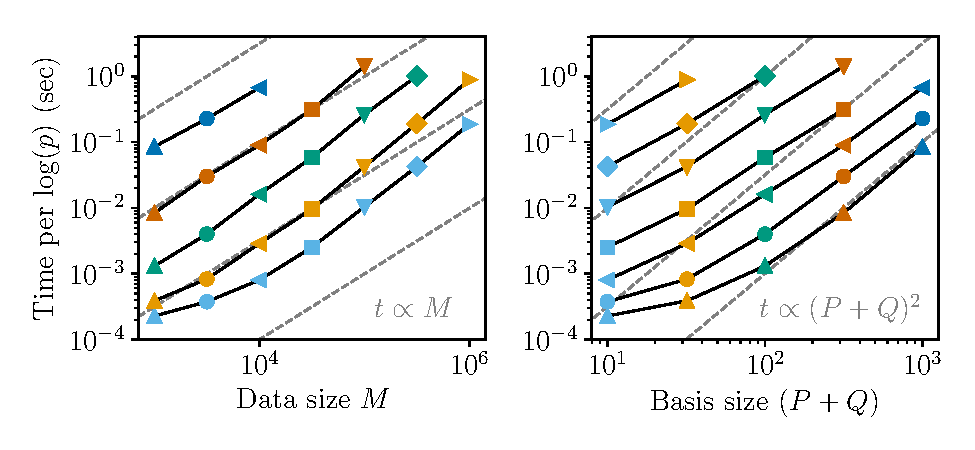
\includegraphics{uncorr_no_L_scaling.pdf}
  \caption{Computation time of the marginal log-likelihood (Equations \ref{eqn:proper-prior-marginal} and \ref{eqn:improper-prior-marginal}) when the data covariance matrix $\vx{K}$ is diagonal and $\vx{L}$ is the identity mapping as a function of dataset size $M$ (left panel) and basis size $P+Q$ (right panel). Values with the same marker shape were computed at the same dataset size $M$. Values with the same marker color were computed at the same dataset size $P+Q$. Polynomials of the form given in the bottom right corner of each panel are shown as dashed gray lines.}
  \label{fig:uncorr-no-L-logp}
\end{figure}

\begin{figure}
  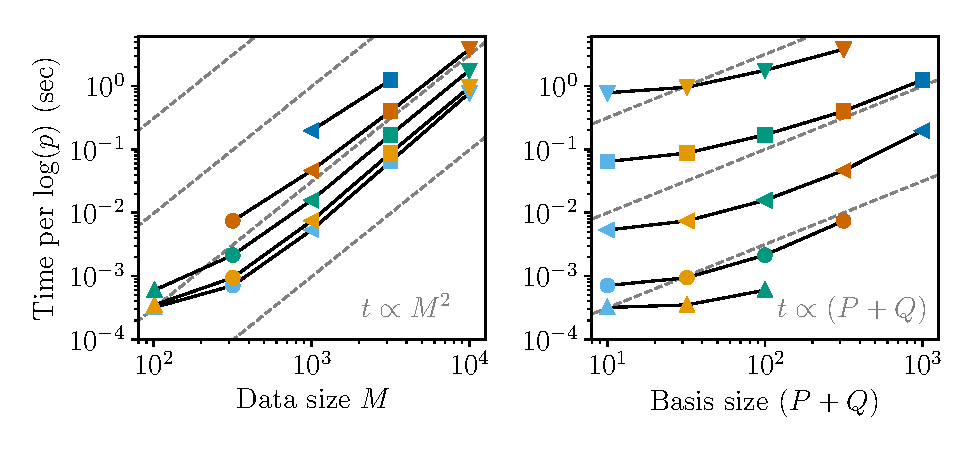
\includegraphics{corr_yes_L_scaling.pdf}
  \caption{Computation time of the marginal log-likelihood when the data covariance matrix $\vx{K}$ is not diagonal and $\vx{L}$ is a dense matrix. See caption of Figure \ref{fig:uncorr-no-L-logp} for a description of figure elements.}
  \label{fig:corr-yes-L-logp}
\end{figure}

\begin{figure}
  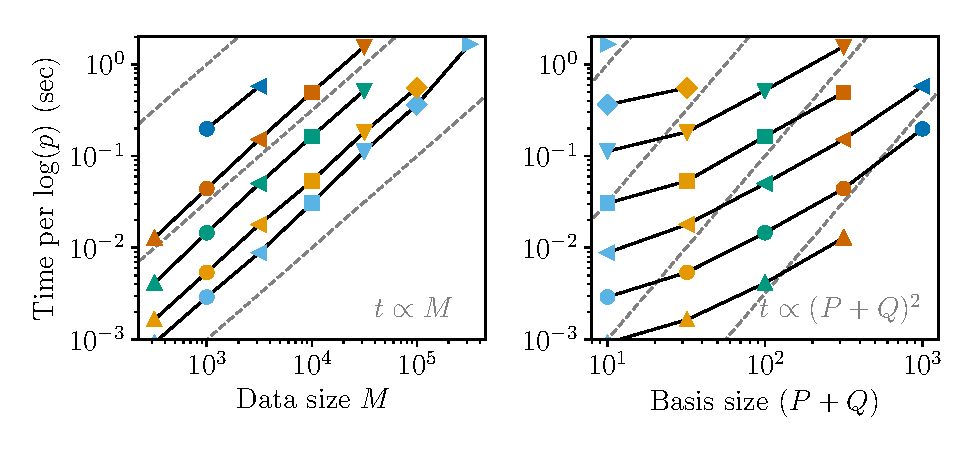
\includegraphics{uncorr_sparse_L_scaling.pdf}
  \caption{Computation time of the marginal log-likelihood when the data covariance matrix $\vx{K}$ is diagonal and $\vx{L}$ is a sparse, banded matrix. See caption of Figure \ref{fig:uncorr-no-L-logp} for a description of figure elements.}
  \label{fig:uncorr-sparse-L-logp}
\end{figure}


\subsection{Test case: multiple absorption lines}
\label{subsec:multiple-absorption-line-test-case}

\begin{figure}
  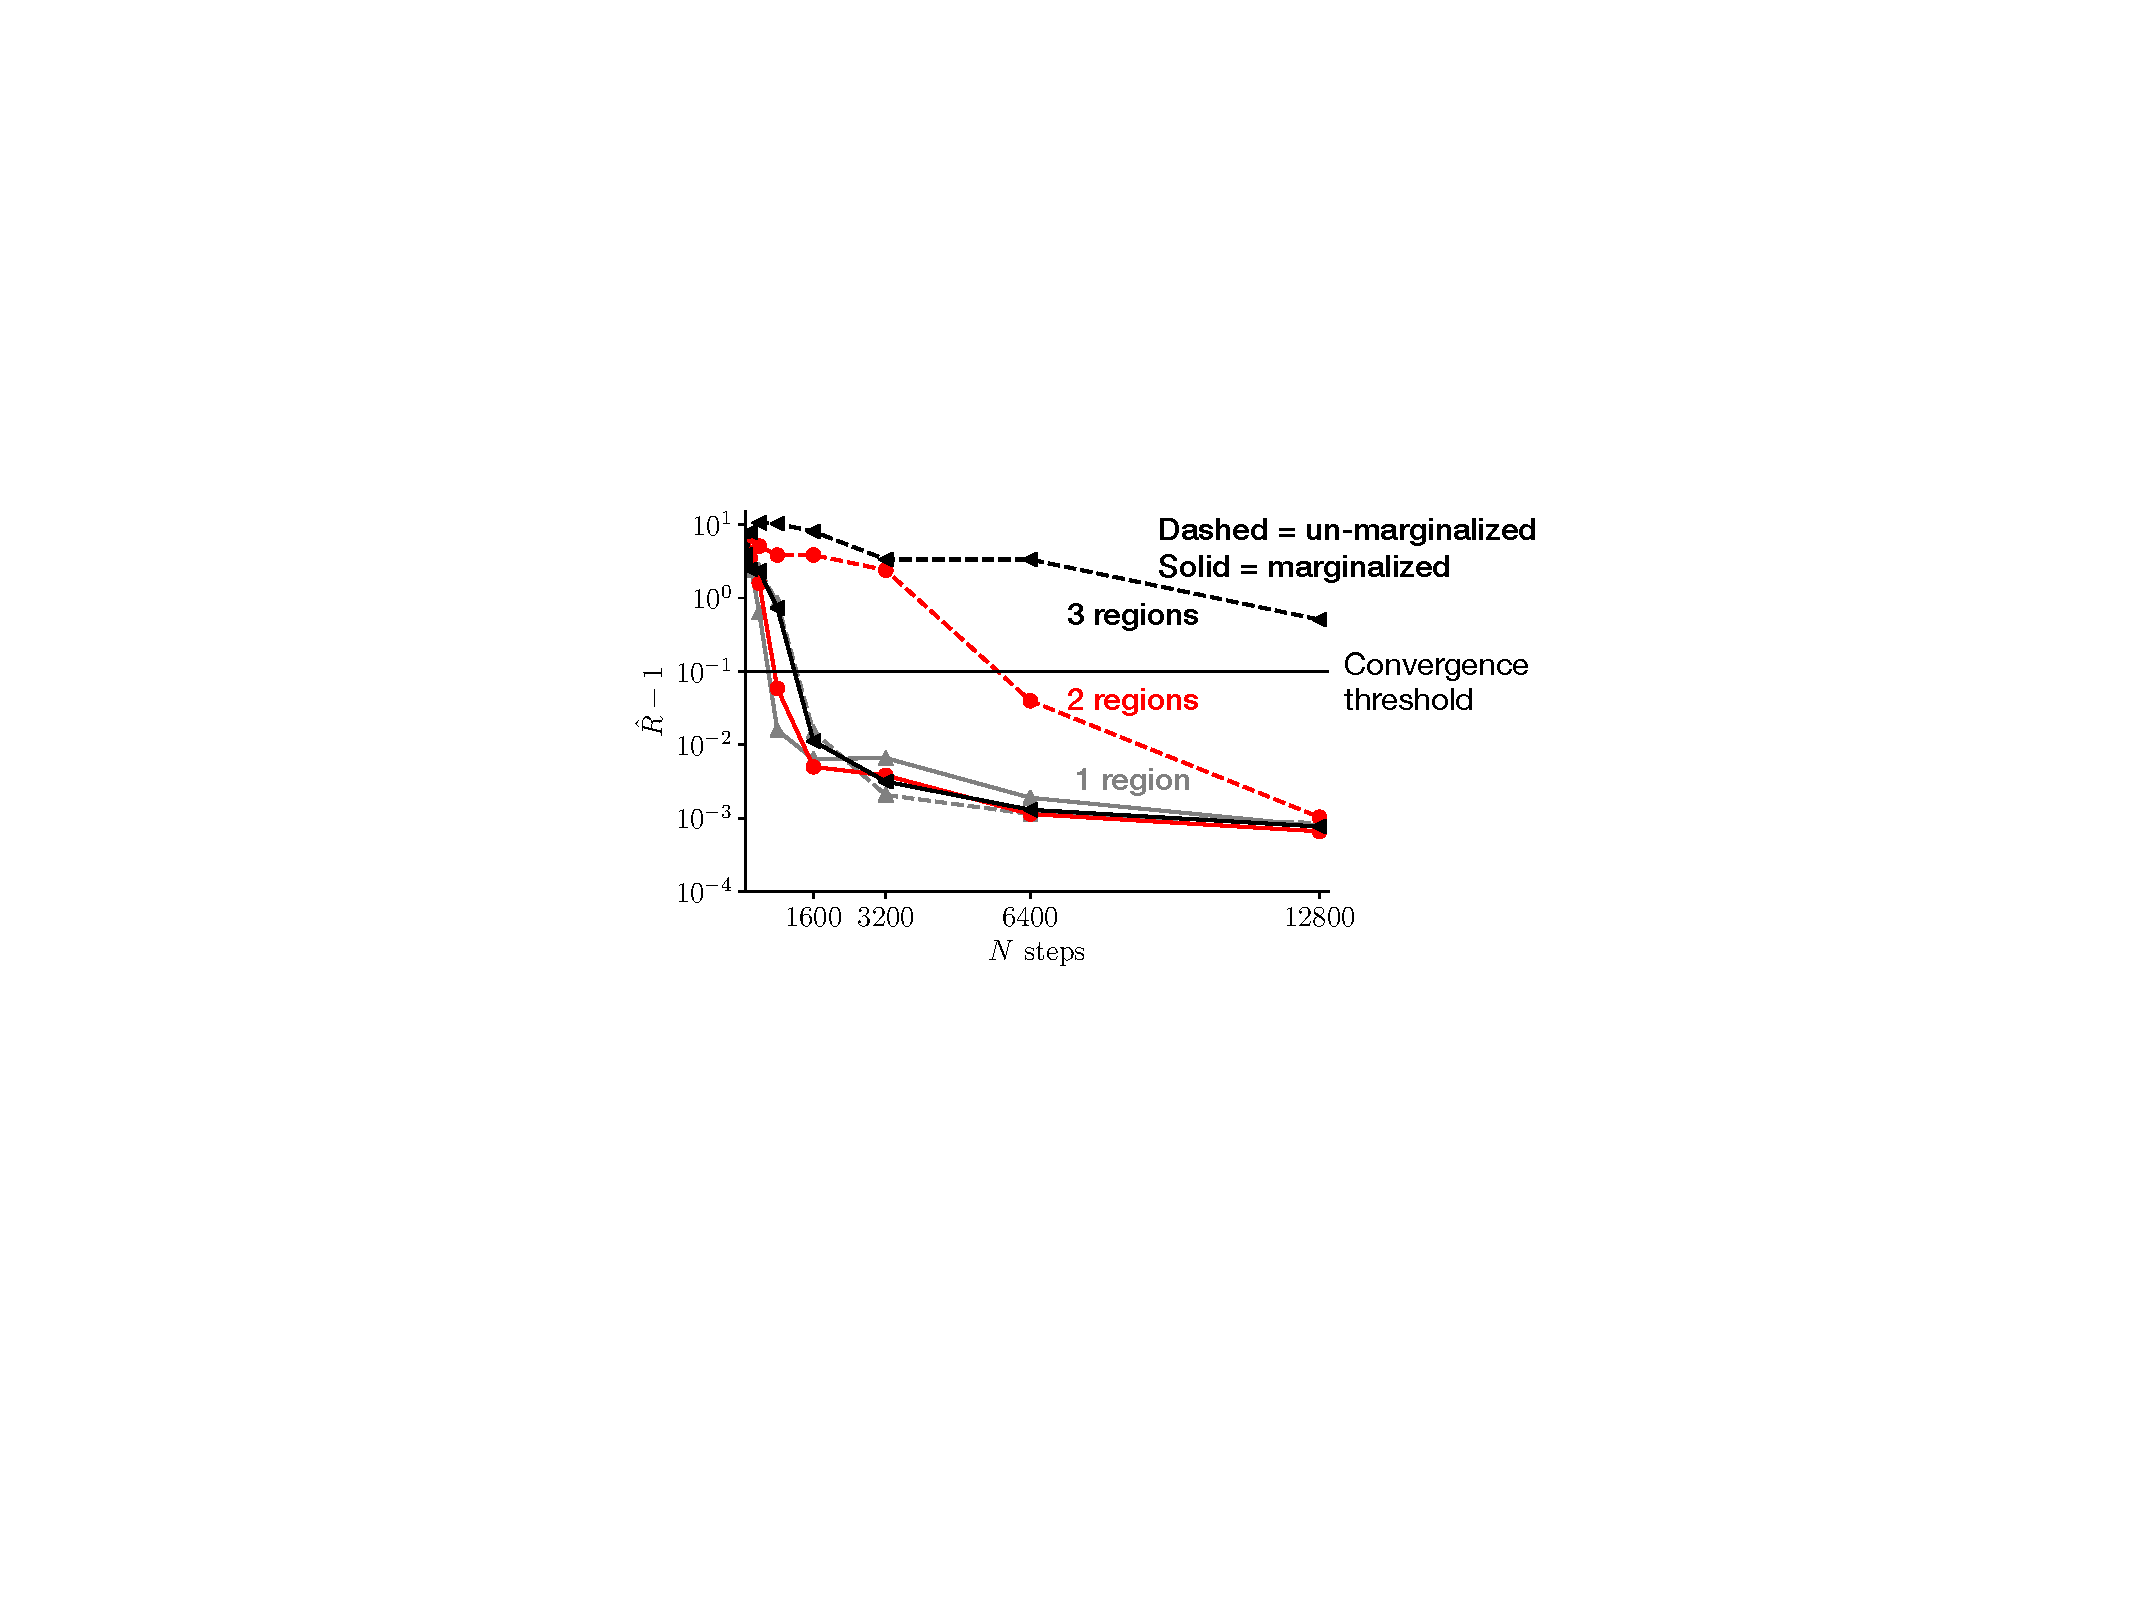
\includegraphics{convergence.pdf}
  \caption{Rubin-Gelman statistic}
  \label{fig:convergence-comparison}
\end{figure}

\begin{figure}
  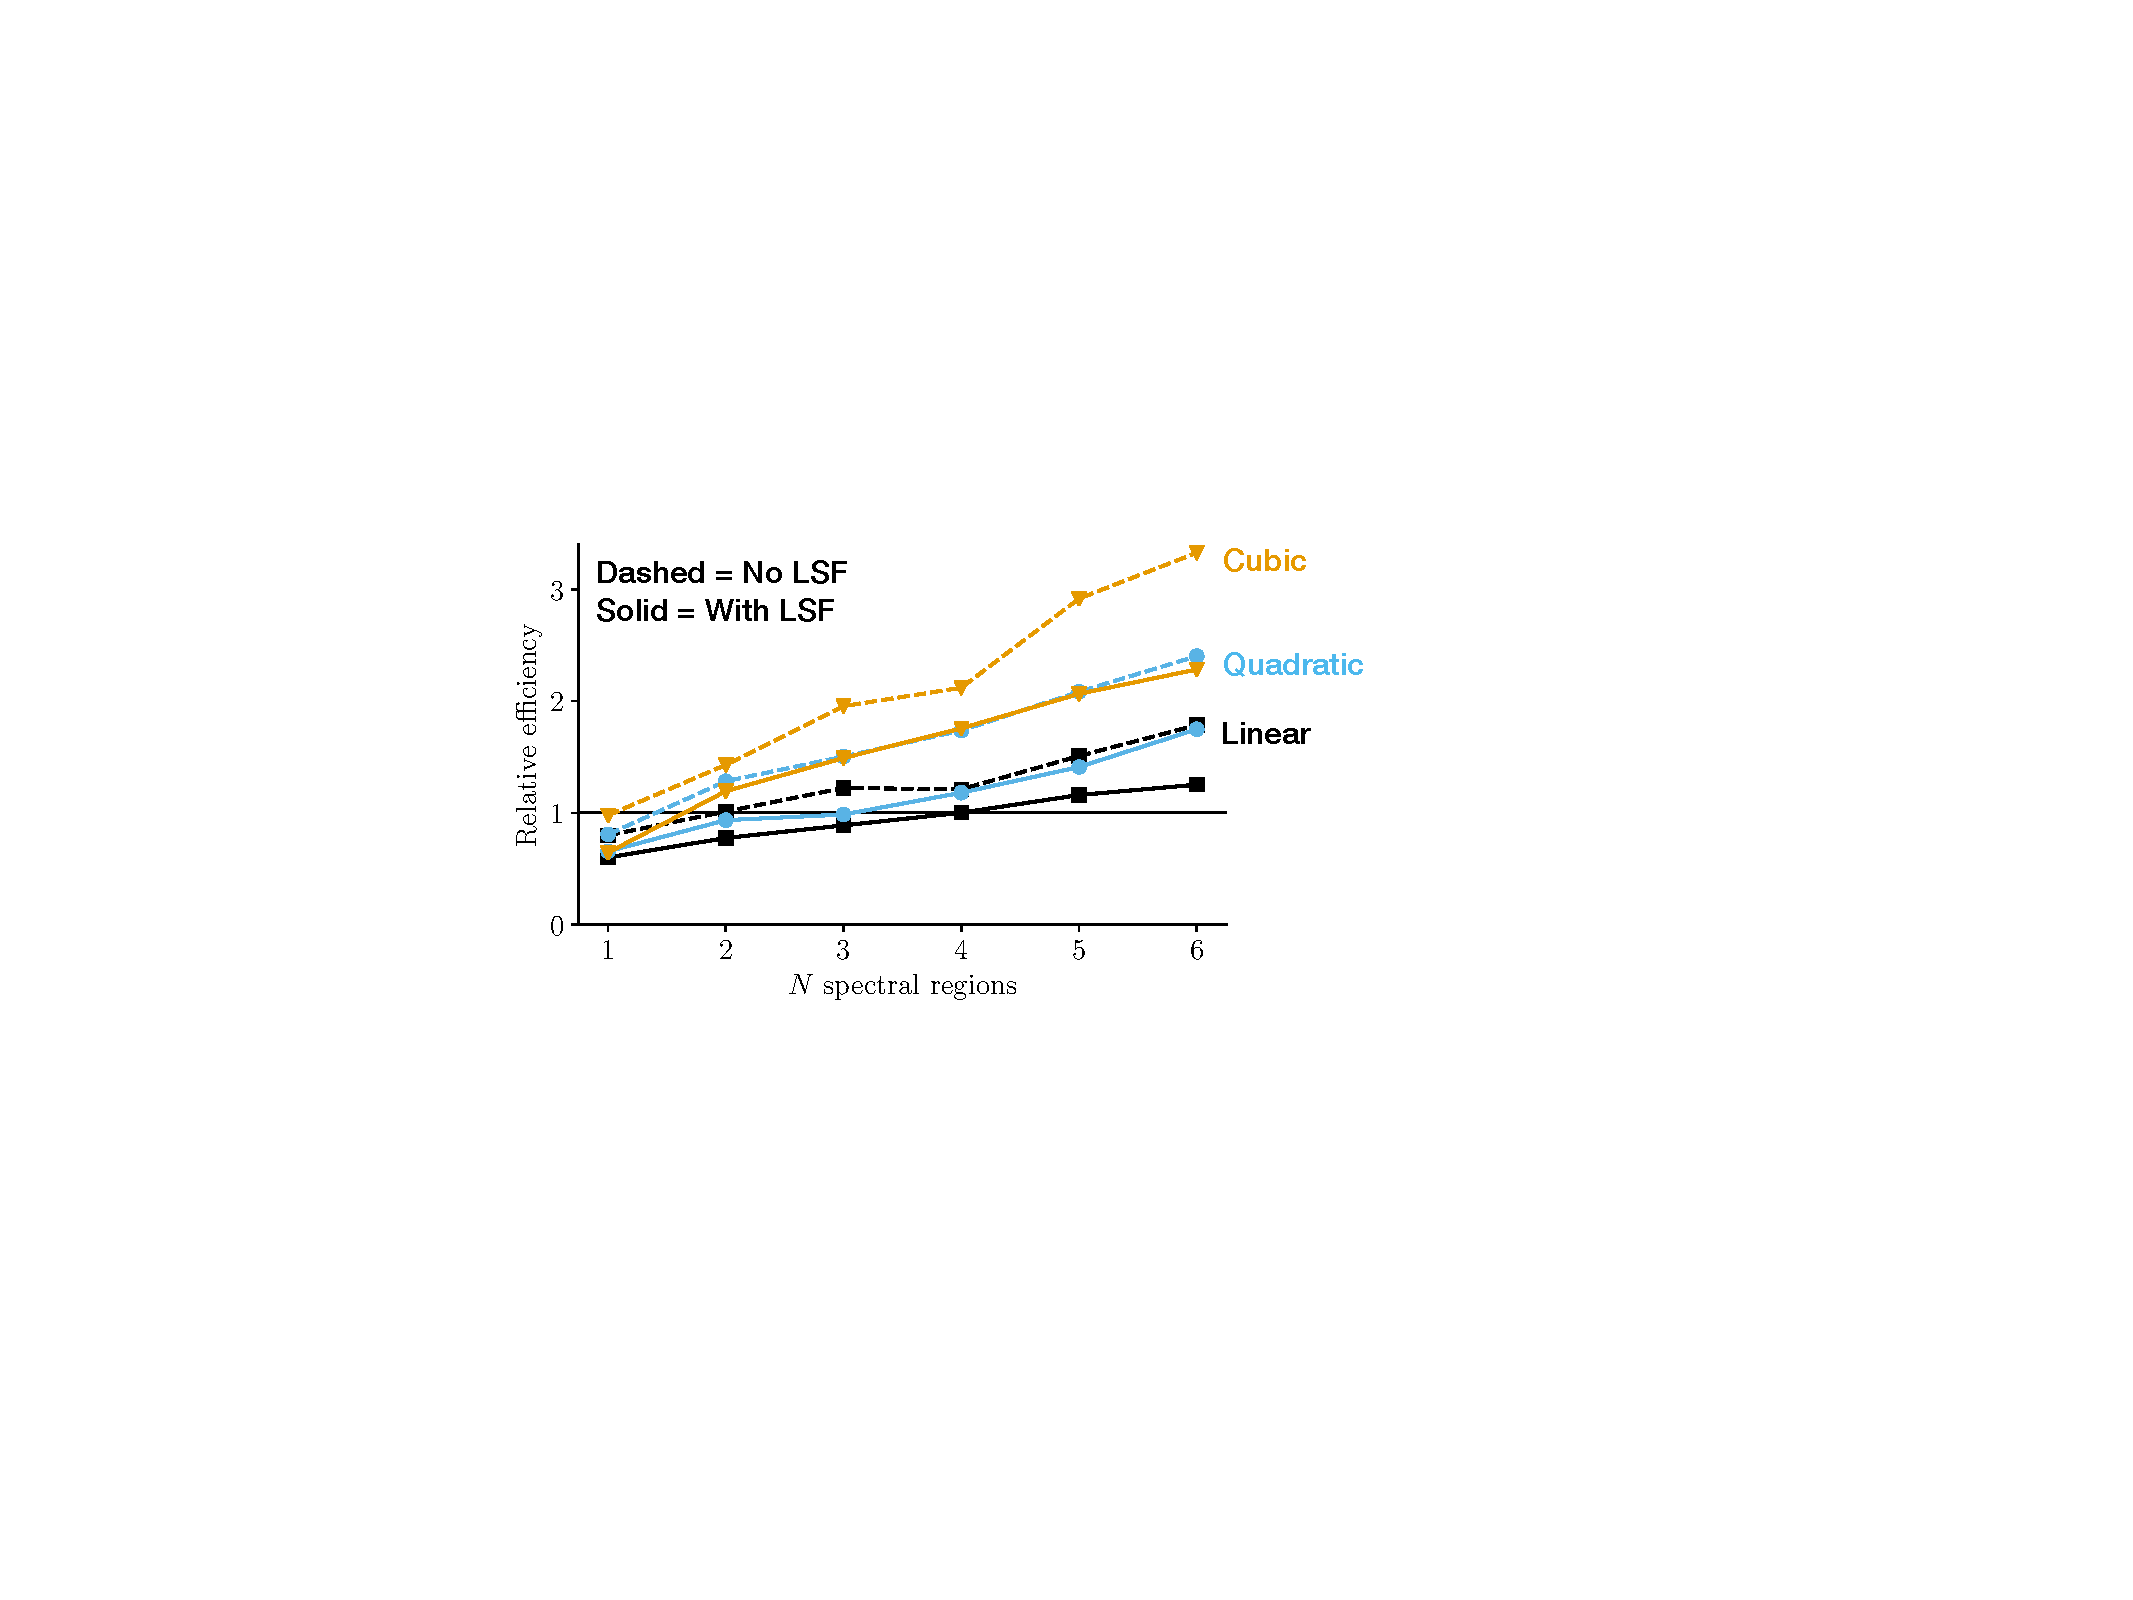
\includegraphics{efficiency.pdf}
  \caption{Independent samples per second}
  \label{fig:efficiency-comparison}
\end{figure}

Motivate and pose the problem
In ISM absorption spectra, it is common to have multiple lines in a spectrum with shared parameters
These lines can be from the same species, e.g. the Lyman series, or from different species, e.g. from Mg\small{I}, Zn\small{II}, and Cr\small{II} in the near ultraviolet.
When these lines are in different regions in a spectrum, each region needs its own continuum parameters; this is the case in which BayesVP does not allow the inclusion of continuum parameters in inference.
This is one of the scenarios in which analytic marginalization can be more efficient than MCMC marginalization

We compare the two methods on how quickly MCMC done using each converges and how efficient MCMC done using each is post-convergence.
Which comparison is more informative for choosing which method to use will depend on the purpose of the MCMC run.
If the goal of an MCMC run is to estimate some value at low-to-moderate precision, the rate of convergence will be the more important factor.
If the goal is to estimate some value at high precision, the burn-in period will usually be a small fraction of the total chain and post-convergency efficiency will be more important.

We consider a case where there are $N$ absorption lines with shared velocity structure, i.e. central velocity and velocity width, but with different amplitudes.
Each absorption line is in a different spectral region.
The continuum in each spectral region is a polynomial of order $M$.
The marginalized likelihood has $2 + N$ absorption line parameters.
The unmarginalized likelihood has $2 + N$ absorption line parameters and $N \times M$ continuum parameters.
We use the \texttt{emcee} implementation of the Goodman and Weare affine-invariant MCMC ensemble sampler to generate draws from the posterior corresponding to each of these likelihoods.
We use the minimum number of `walkers,` which is twice the number of parameters.


We use the Rubin-Gelman statistic $\hat{R}$ CITEP to assess convergence.
We run ten MCMC instances for 12800 (per-walker) steps and compute the Rubin-Gelman statistic from the second half of sub-chains of length $2^p \times 100$ for $p=0, 1, \ldots, 7$.
$\hat{R}$ is computed separately for each parameter.
Following common usage, we consider convergence to be reached when the $\hat{R}$ of all parameters is less than $1.01$.
We run this test for 1, 2, and 3 regions and absorption lines assuming a continuum of order 1, i.e. a straight line.
The value of the $\hat{R}$ as a function of (total) number of steps is shown in Figure \ref{fig:convergence-comparison}.
When there is a single region and line, the MCMC marginalization chain takes twice as many steps as the analytic marginalization chain to converge; when there are two regions, it takes eight times as many steps; when there are three, the MCMC marginalization  chain has not converged by the maximum chain length of 12800 while the analytic marginalization chain converges within 1600 steps.

We use the number of independent samples per unit time to assess efficiency.
We run MCMC with the marginalized likelihood for 2000 burn-in steps and 8000 converged steps and record the average time per sample, $t_s$
Because MCMC with the unmarginalized likelihood takes many steps to converge, we use draws from the converged part of the marginalized likelihood chain as a starting point
These draws only have values for the absorption line parameters
At each set of absorption line parameters, we sample a set of continuum parameters from the conditional distribution discussed in Section \ref{subsec:conditionals}
From this starting point, we run MCMC with the unmarginalized likelihood for 4000 burn-in steps and 36000 converged steps and record the average time per sample
We then compute the average integrated autocorrelation times $\tau_f$ of the walkers in both chains.
The number of independent samples per unit time is $n_i = \left(\tau_f \, t_s \right)^{-1}$.

We compute $n_i$ for a number of regions $N = 1, 2, \ldots, 6$, continua of polynomial order $M=$ 1, 2, and 3, and either a trivial LSF or a banded LSF.
The ratio $n_i^{\text{marg}} / n_i^{\text{unmarg}}$ for each of these cases is shown in Figure \ref{fig:efficiency-comparison}.
When this ratio is greater than 1, running MCMC with the marginalized likelihood for a fixed amount of time will produce more independent samples than running MCMC with the unmarginalized likelihood for the same amount of time.
The greater the number of regions and the order of the continuum, the greater the efficiency advantage of the marginalized likelihood over the unmarginalized likelihood.
This advantage will not depend on the number of datapoints in each spectral region so long as the LSF is trivial or banded, since the evaluation time of both likelihoods grows linearly with dataset length (see Section \ref{subsec:scaling}).

\subsection{Marginalization over continuum parametrizations}
\label{subsec:contparametrization-marginalization}
you can trivially marginalize over what the continuum is when you have analytics.
you can't really do that if you don't marginalize simultaneously and it's very hard to marginalize without analytics.
why is that? so many parameters.
time cost is manageable and "linear."

advantages of marginalizing over continuum parametrizations are different in different use cases.
just very complicated continua (such as that exceptionally wacky HSLA one or one of the confusing ones from my 2015 depletion paper), where it's hard to qualitatively say "this is the right model" and you just actually want to consider the possibility of different parametrizations.

automation of spectral analysis.
big absorption line surveys of all sorts going on right now; also analysis of synthetic observations.
can't manually look at all of them!!
therefore, need way of automatically selecting continuum complexity; marginalization is an easy way to go.

example one (only example?): generate simple spectra with continua of different orders, fit lines with assumed orders vs. marginalization over orders

\section{Discussion}
\label{sec:discussion}
The main weakness of the analytic marginalization formulas used in this package are the restrictive and unphysical assumptions that the formulas require.
The un-marginalized likelihood function is required to be Gaussian.
Even just among types of dataset in which absorption lines can be found, this is not always a justifiable assumption.
In particular, it does not apply to data where photon counts are small enough that the Gaussian approximation to the Poisson distribution is inappropriate.
This package should be used with caution when analyzing X-ray spectra, for example.

The linear nuisance parameters also cannot be bounded in any way.
This is assumption is needed because integrals of the multivariate normal distribution over finite regions must be computed numerically.
While numerical integration methods tailored specifically for this problem exist \citep{Genz:2009jp}, they are still much slower than the analytic integral over infinite regions.
Unbounded MLNPs are often obviously unphysical.
Stars never emit negative light but an unbounded MLNP description of a stellar continuum allows this possibility.
This assumption can be particularly dangerous when the basis is physically motivated.
The contribution of different stellar population templates to the spectrum of a galaxy, for example, should always be non-negative.
Otherwise, the templates can be combined in a way that could not actually happen.

\subsection{What do the tests really tell you}

All of these tests were done using the \texttt{emcee}.
We chose to use \texttt{emcee} because it is very commonly used astronomy in general and in Bayesian absorption line analysis packages in particular.
More sophisticated or problem-specific proposal methods could potentially reduce the advantage of analytic marginalization over MCMC marginalization in terms of convergence rate and efficiency.
One advantage of analytic marginalization over this solution is that it is very easy to add analytic marginalization to existing analysis code --- only the actual likelihood calculation step needs to be modified.


\section{Conclusion}
\label{sec:conclusion}
have a package that computes marginal likelihoods and their gradients
idea of marginalizing out linear parameters is not entirely new -- done in the Joker and we independently did it (over a finite range because we had just one MLNP) in these other two papers.
the new stuff is: including something analogous to an LSF, calculating the derivatives, providing a general use package

have shown that this package is fast enough to use over a range of dataset sizes, provides certain benefits
package was designed to solve continuum problem, but applicable to a number of other things


\acknowledgments

\software{emcee \citep{2013PASP..125..306F},
numpy \citep{vanderWalt:dp},
matplotlib \citep{2007CSE.....9...90H}
}

\bibliography{bibliography.bib}

\end{document}
